\section{Methodology}\label{sec:methology}

\subsection{Dataset}\label{subsec:dataset}

In our project, we utilized the \emph{Human Activity Recognition Using Smartphones} dataset, referenced in our literature as~\cite{misc_human_activity_recognition_using_smartphones_240}.
This database is built from recordings of 30 subjects performing activities of daily living (ADL) while carrying a waist-mounted smartphone with embedded inertial sensors.

It was sourced from a diverse group of 30 volunteers aged 19--48; the dataset captures six common activities: walking, walking upstairs, walking downstairs, sitting, standing, and laying.
Each subject wore a Samsung Galaxy S II smartphone on the waist, enabling the capture of 3-axial linear acceleration and 3-axial angular velocity at a 50Hz rate.
The dataset, a multivariate time-series collection in the computer science domain, is suitable for tasks such as classification and clustering.

Instead of the raw time-series data, we utilized the processed features of the \emph{Human Activity Recognition Using Smartphones} dataset.
The dataset provided a comprehensive set of features derived from the accelerometer and gyroscope sensors, which were more aligned with our project objectives.

These features include various statistical measures estimated from the processed sensor signals such as but not limited to mean, standard deviation, median absolute deviation as well as frequency domain features derived from the Fast Fourier Transform (FFT).
In total, the dataset provided 561 features for each sample.
Which of these features were used in our project is discussed in Section~\ref{subsec:preprocessing}.

The authors of the dataset also provided a partitioned dataset, which was split into two sets: a training set and a test set.
The training set consists of 70\% of the data, while the test set consists of the remaining 30\%.
Which comes to 7352 and 2947 samples respectively.

The authors also provide a short YouTube video \cite{youtube_recording_of_the_experiment_240} that shows the data collection process.
This video shows that the data was collected by having the subjects perform the activities while wearing the smartphone on their waist.
The subjects were also asked to perform the activities multiple times, which is why the dataset contains multiple samples for each subject and activity.

\subsection{Data Exploration}\label{subsec:data-exploration}

In machine learning, it is important to understand the data you are working with, since this can help you decide which features to use and which machine learning approach to use.
Therefore, we analyzed the dataset with plots to get a better understanding of the data we were working with.

Since looking at all the features was not feasible, we decided to only look at features that had less than 10\% correlation with other features.
Doing this ensures that we look at features that had the least amount of redundancy and should therefore be the most informative.

Figure~\ref{fig:pairplot} shows a pair-plot of the features we decided to look at.
A pair-plot shows a scatterplot for each feature combination, as well as histograms of the features along the diagonal.
From the pair-plot, we can see that there are some features that could be used to distinguish between a few classes.
The features \texttt{tBodyAcc-std()-X} and \texttt{tBodyAcc-correlation()-X,Z}, for example, show a good separation between the different \texttt{WALKING} activities and the more stationary activities.

\begin{figure}[ht]
    \centering
    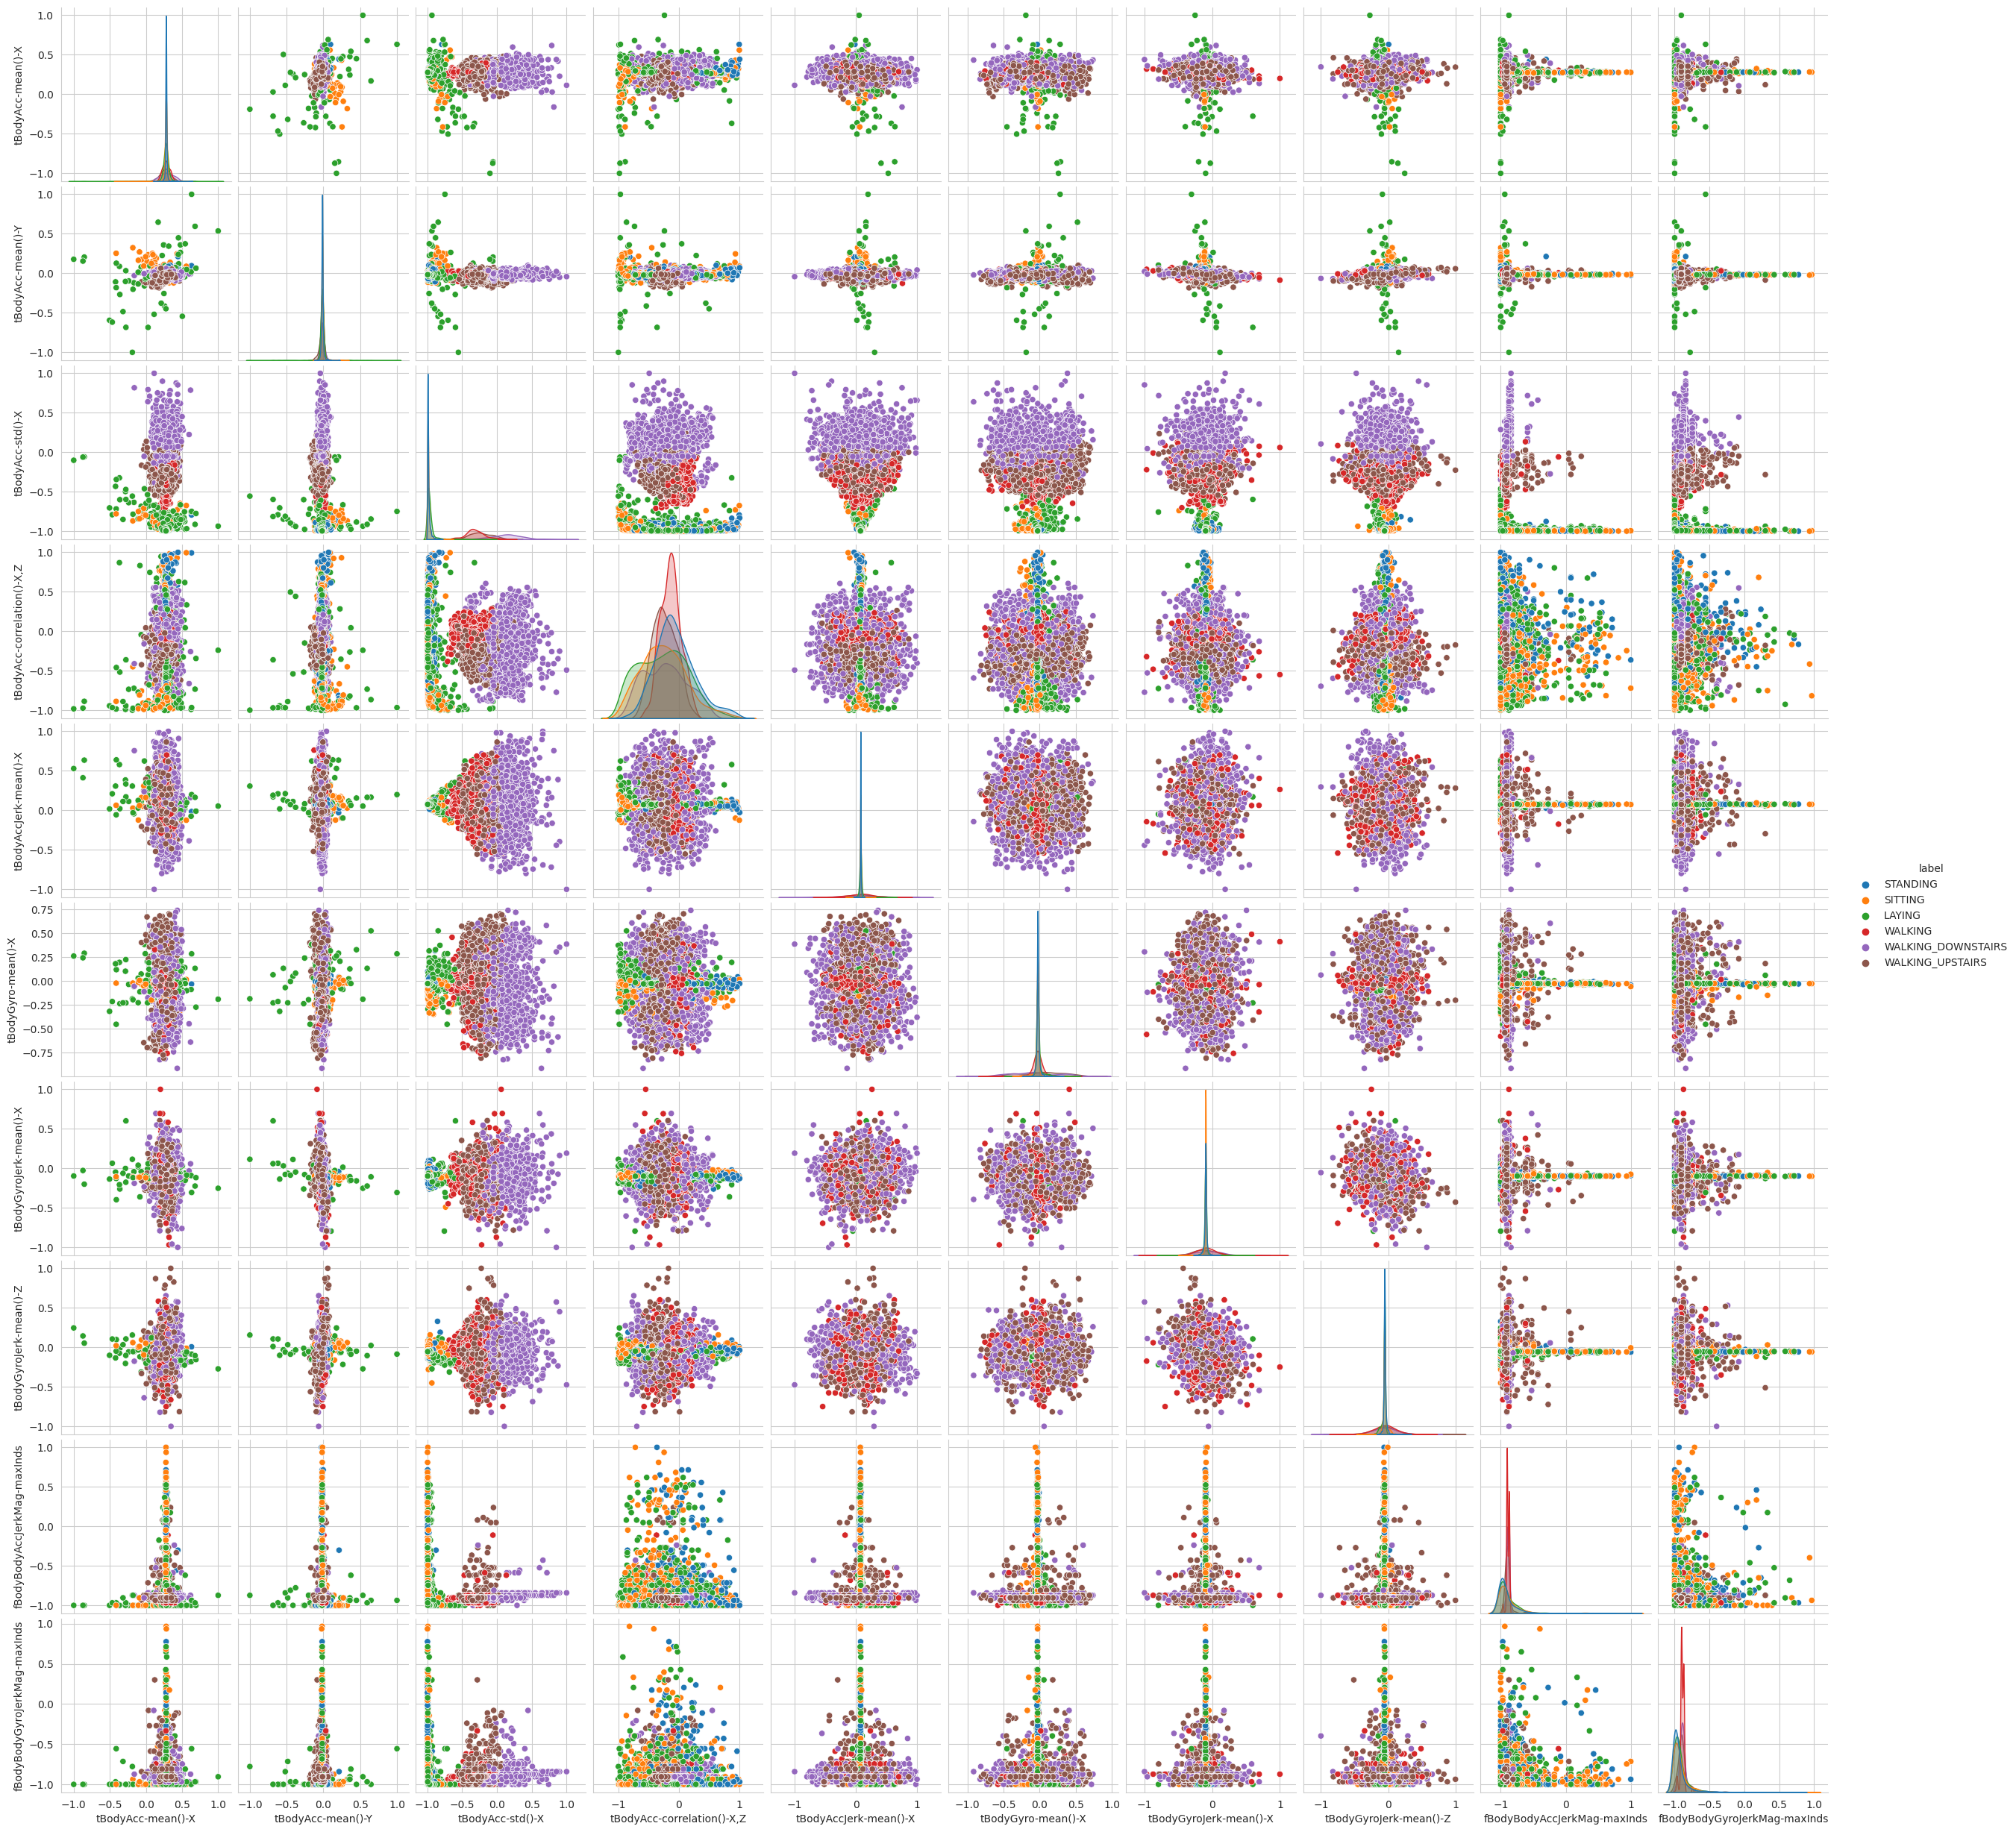
\includegraphics[width=\textwidth]{./img/pairplot}
    \caption{Pairplot of highly uncorrelated features}
    \label{fig:pairplot}
\end{figure}

This is further confirmed by looking at the boxplot in Figure~\ref{fig:boxplot}, which shows the distribution of the features for each class, and the feature \texttt{tBodyAcc-std()-X} also shows a good separation between the stationary activities and the \texttt{WALKING} activities.
The boxplot further shows that some features have little variance, such as \texttt{tBodyBodyGyroJerkMag-maxInds}, which has a small interquartile range and a lot of outliers.
The feature \texttt{tBodyAcc-correlation()-X,Z} on the other hand shows a strong overlap between the classes, which is not surprising since it is a correlation between two features that are already used to distinguish between the classes.

\begin{figure}[ht]
    \centering
    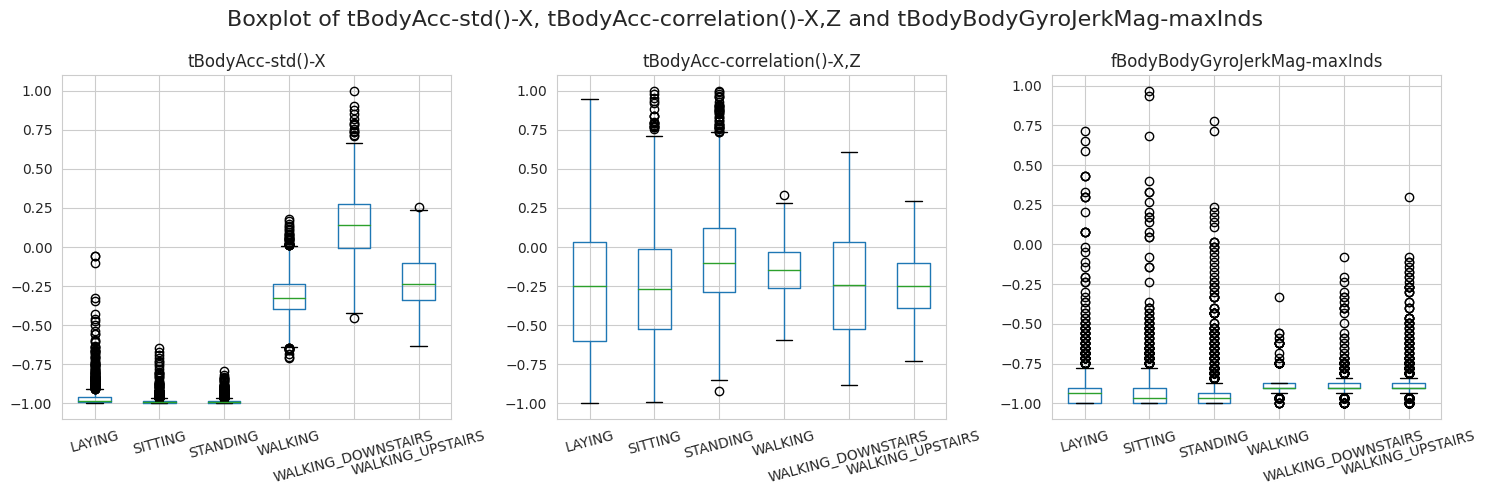
\includegraphics[width=\textwidth]{./img/boxplot}
    \caption{Boxplot of tBodyAcc-std()-X, tBodyAcc-correlation()-X,Z and tBodyBodyGyroJerkMag-maxInds}
    \label{fig:boxplot}
\end{figure}

The plot that showed the most promise was the line-plot in Figure~\ref{fig:lineplot}, which shows the total acceleration over time in each axis.
This graph shows that the accelerations can definitely be used to distinguish between the different activities, since they have very different patterns with little overlap.
The activity \texttt{LAYING} can be distinguished from the other activities, as it has no overlap with the other activities.
The activities \texttt{SITTING} also shows no overlap with the other activities in the Z-axis and Y-axis, apart from itself.
But the graph even allows us to clearly identify \texttt{STANDING} which has a lot of overlaps in the X and Y-axis, but can still be distinguished from the other activities in the Z-axis.

\begin{figure}[ht]
    \centering
    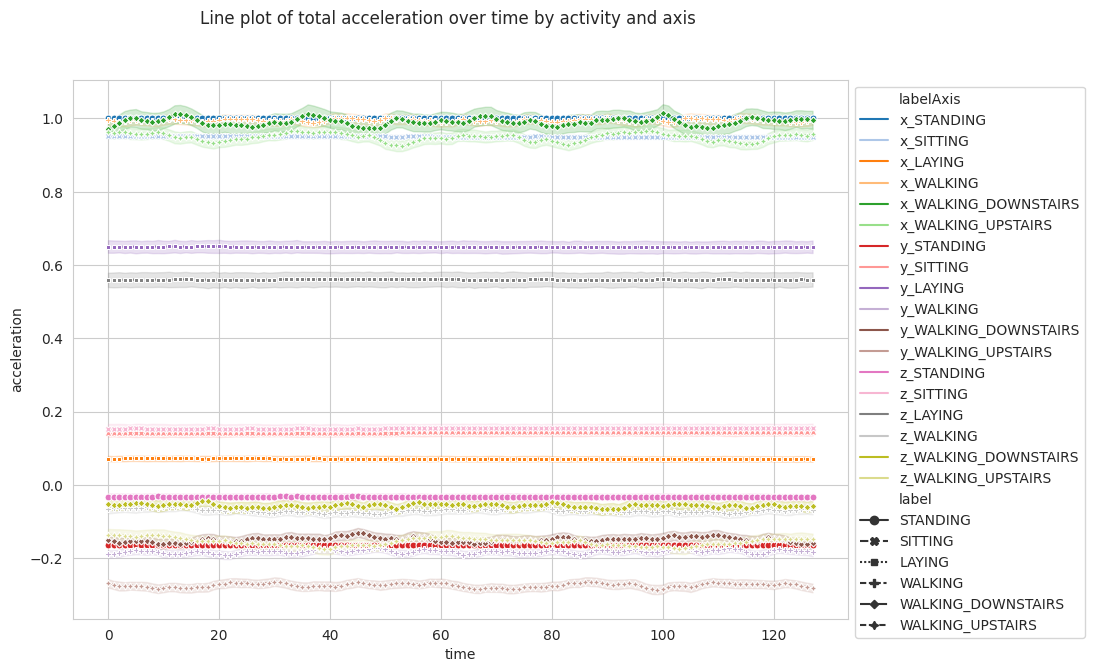
\includegraphics[width=\textwidth]{./img/lineplot}
    \caption{Lineplot of total acceleration over time in each axis}
    \label{fig:lineplot}
\end{figure}

The data exploration showed that the data is definitely separable and can probably also be solved with less complex machine learning approaches.
However, since the focus of the project was on deep learning, we did not explore other machine learning approaches such as knn, decision trees or support vector machines.

\subsection{Preprocessing}\label{subsec:preprocessing}

Since the dataset was already processed, we did not have to perform any preprocessing steps to generate features, but we did some preprocessing to reduce the number of features.

% TODO search for paper to reference for correlation matrix

For this, we used a correlation matrix to find features that were highly correlated with each other.
Features that have a high correlation with each other imply that they are redundant and can be removed.
Redundant features can be removed since the information they provide is already captured by other features.
This reduces the number of features, which in turn leads to models that are less complex, as they need to learn fewer features.

Figure~\ref{fig:cormat-before} shows the correlation matrix before preprocessing, while Figure~\ref{fig:cormat-after} shows the correlation matrix after preprocessing.
As a threshold for removing features, we used a correlation coefficient of \emph{0.95}.
This reduced the number of features from 561 to 253, effectively reducing the number of features by more than half.

\begin{figure}[ht]
    \centering
    \begin{minipage}{0.45\textwidth}
        \centering
        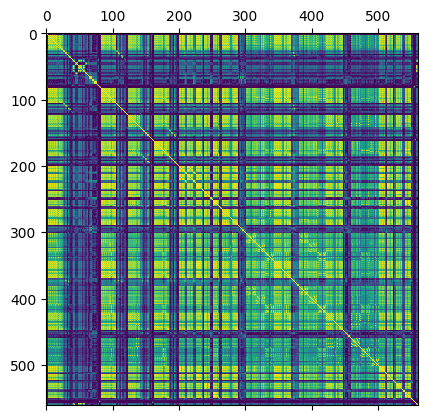
\includegraphics[width=\textwidth]{./img/correlation-matrix-before}
        \caption{Correlation matrix before preprocessing}
        \label{fig:cormat-before}
    \end{minipage}\hfill
    \begin{minipage}{0.45\textwidth}
        \centering
        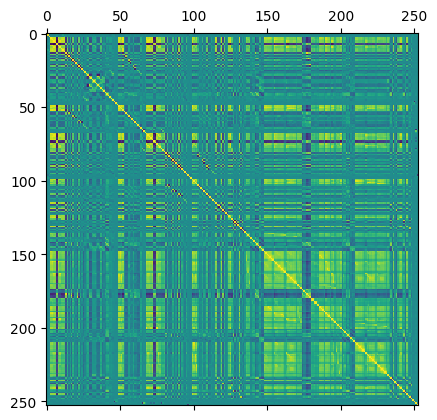
\includegraphics[width=\textwidth]{./img/correlation-matrix-after}
        \caption{Correlation matrix after preprocessing}
        \label{fig:cormat-after}
    \end{minipage}
\end{figure}

We also decided to use the test set provided by the dataset as our held-back test set.
For training, we split the training set into a set used for actual training and a set used for validation.
This was done to be able to evaluate the performance of the model during training, and to ensure that the model did not over fit to the training set.
The validation set was 30\% of the training set, which comes to around 2206 samples for the validation set and 5146 samples for the training set.

\subsection{Architectures}\label{subsec:architectures}

This section discusses the architectures we tried and evaluated in our project.
For different architectures, we tried to first build a simple model, and then a more complex one that where we also tuned the hyperparameters.

\subsubsection{Feedforward Neural Network}

\textbf{Simple Feedforward Neural Network}

Our project initiated with a simple Feedforward Neural Network (FF).
This model consisted of an initial dense layer with 512 units, a hidden dense layer with 128 units using the ReLU activation function, and an output dense layer with 6 neurons.
This was the simplest model we could think of.
Figure~\ref{fig:fnn-simple-architecture} shows a visualization of the simple Feedforward Neural Network.

\begin{figure}[ht]
    \centering
    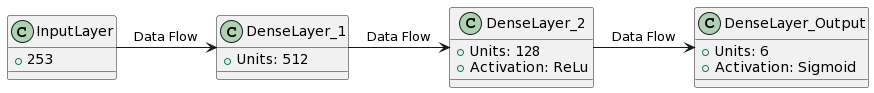
\includegraphics[width=\textwidth]{./img/ffnn/simple/fnn-simple-architecture}
    \caption{Visualization of simple Feedforward Neural Network architecture}
    \label{fig:fnn-simple-architecture}
\end{figure}

\textbf{Tuned Complex Feedforward Neural Network}

The results from the simple Feedforward model were already pretty good, but we wanted to see if we could improve the performance by increasing the complexity of the model and tuning the hyperparameters.
For this, we utilized Keras Tuner, employing a RandomSearch strategy.
This approach allowed us to automatically fine-tune the hyperparameters of our model.
Figure~\ref{fig:fnn-tunable-neurons} shows the network and what parameters are tunable, such as the number of layers, the number of units in each layer and the dropout rate.
The goal was to identify the most effective configuration for our dataset, enhancing the model's performance.

\begin{figure}[ht]
    \centering
    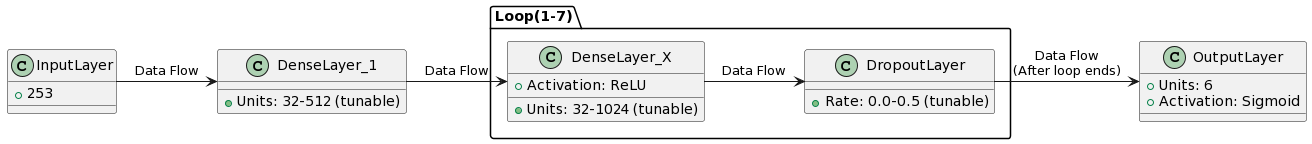
\includegraphics[width=\textwidth]{./img/ffnn/tuned/fnn-tunable-neurons}
    \caption{Visualization of tunable Feedforward Neural Network architecture}
    \label{fig:fnn-tunable-neurons}
\end{figure}

\subsubsection{Convolutional Neural Network}

\textbf{Simple Convolutional Neural Network}

We also developed a Convolutional Neural Network model, comprising convolutional layers, max pooling, global max pooling, a dropout layer for regularization, and a softmax output layer.
While such models are typically used for image classification, we wanted to explore whether they could be used for time-series classification as well.
This also did not need any real preprocessing apart from reshaping the data to fit the input shape of the network.
Figure~\ref{fig:cnn-simple-architecture} shows a visualization of the simple Convolutional Neural Network.

\begin{figure}[ht]
    \centering
    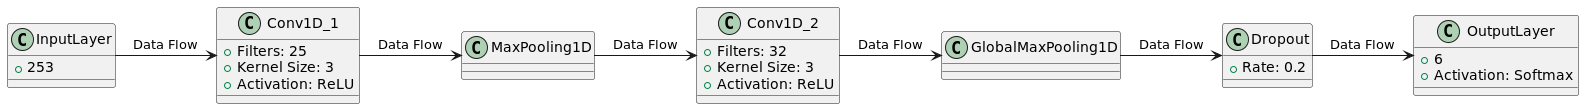
\includegraphics[width=\textwidth]{./img/cnn/simple/cnn-simple-architecture}
    \caption{Visualization of simple Convolutional Neural Network architecture}
    \label{fig:cnn-simple-architecture}
\end{figure}

\textbf{Tuned Convolutional Neural Network}
While the simple Convolutional Neural Network model performed well, we still wanted to explore whether we could improve its performance by tuning its hyperparameters.
This involved tuning the number of filters in the convolutional layers and the dropout rate, as shown in Figure~\ref{fig:cnn-tunable-filters}.

\begin{figure}[ht]
    \centering
    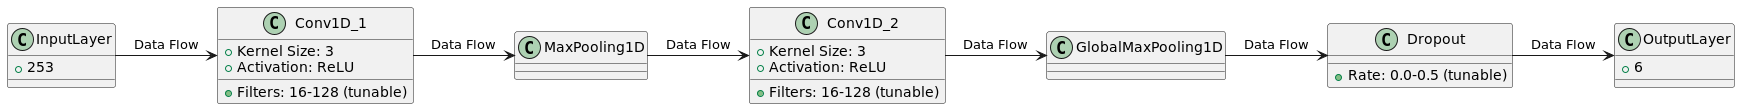
\includegraphics[width=\textwidth]{./img/cnn/tuned/cnn-architecture}
    \caption{Visualization of tunend Convolutional Neural Network architecture}
    \label{fig:cnn-tunable-architecture}
\end{figure}

\subsubsection{Long Short-Term Memory}

We wanted to also try classification by using the windowed time series values instead of the processed features.
We decided to try a Long Short-Term Memory (LSTM) model, which is a type of Recurrent Neural Network (RNN) that is commonly used for time series classification.
We did not tune the hyperparameters of this model, since we wanted to see how well it would perform without tuning.

\subsubsection{Transformer}

Since transformers are currently very popular in the field of natural language processing, we wanted to see if they could also be used for time series classification.
Again, we did not tune the hyperparameters of this model to see how well it would perform without tuning.

\subsection{Training}\label{subsec:training}

As mentioned in Section~\ref{subsec:preprocessing}, we split the training set into a training set and a validation set.
The validation set was used to evaluate the performance of the model during training, and to ensure that the model did not over fit to the training set.

We trained every model for 100 epochs and used five trials for the Keras Tuner with 3 models per trial, so we tuned a total of 15 models for each model we tuned.
For the models, we tuned, we used \texttt{RandomSearch} as the tuner and optimized for validation accuracy.

\subsection{Evaluation}\label{subsec:evaluation}

For models that were tuned, we retrained the model with the best score on the training set and evaluated it on the test set.
This was done to plot the accuracy and loss graphs for the tuned models.

For evaluating the performance of the models, we used the test set provided by the dataset.
This is also commonly referred to as the held-back test set, since it is not used during training or validation.
Having a held-back test set is important since it allows us to evaluate the performance of the model on unseen data.

For evaluating the models, we used the accuracy, precision, recall and F1-score, as well as the confusion matrix.
These metrics are commonly used for classification tasks, and they allow us to evaluate the performance of the model on a per-class basis.